\subsection{TracTrac}
\label{sec:locate:tractrac}

TracTrac~\cite{tractrac} is a fast Python software written by Joris Heyman, to track generic moving objects.

\subsubsection{Algorithm}

The detection is performed by means of DoG and LoG filters, together with Shi-Tomasi corner detection.
Then, a subpixel refinement is applied

\subsubsection{Evaluation}

The only output obtained from the script was an image like figure~\ref{fig:locate:tractrac} for each frame.
No numeric coordinate could be extracted from the execution, nor it was possible to understand the bubbles' positions from the output.
On top of that, the speed was also extremely low (1 FPS), despite selling as ``very fast software, that can track 10~000 particles per second''.

\begin{figure}
	\centerline{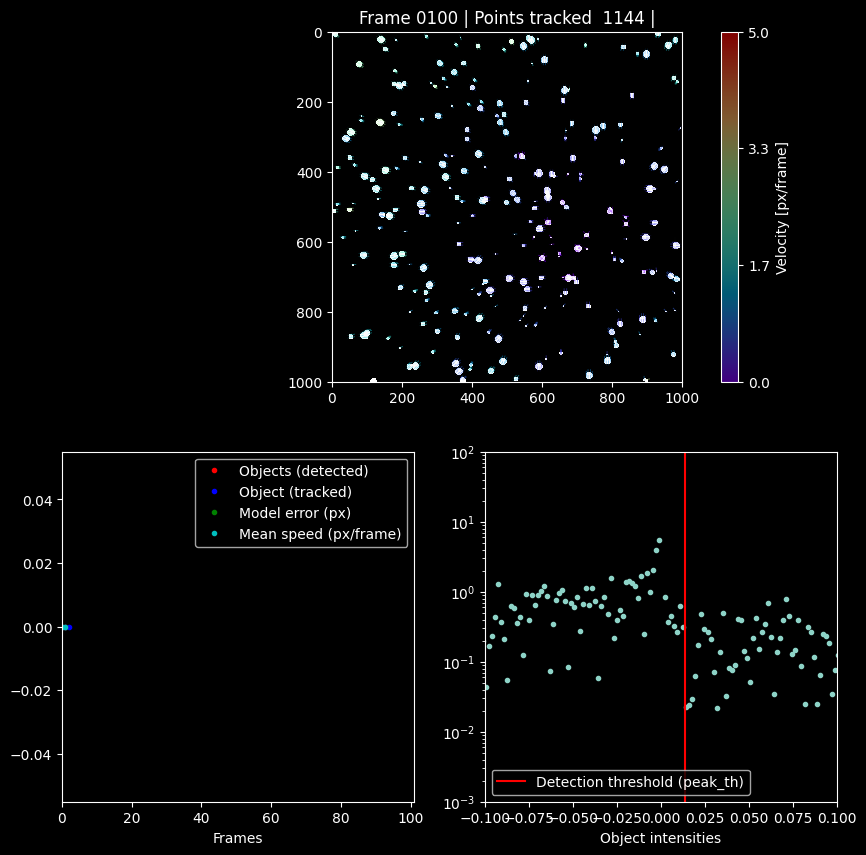
\includegraphics[width=0.7\textwidth]{images/locate/tractrac.png}}
	\caption{\centering TracTrac's result}
	\label{fig:locate:tractrac}
\end{figure}
